% Design

\section{Design}
% TAKEAWAY 1: The reader should be able to see the logical divisions in the Syndicate architecture, and how they fit together. 
% \\
% TAKEAWAY 2: The reader should see why we made the architectural decisions we did, given our requirements and constraints.
% \\

\begin{figure}[h!]
\centering
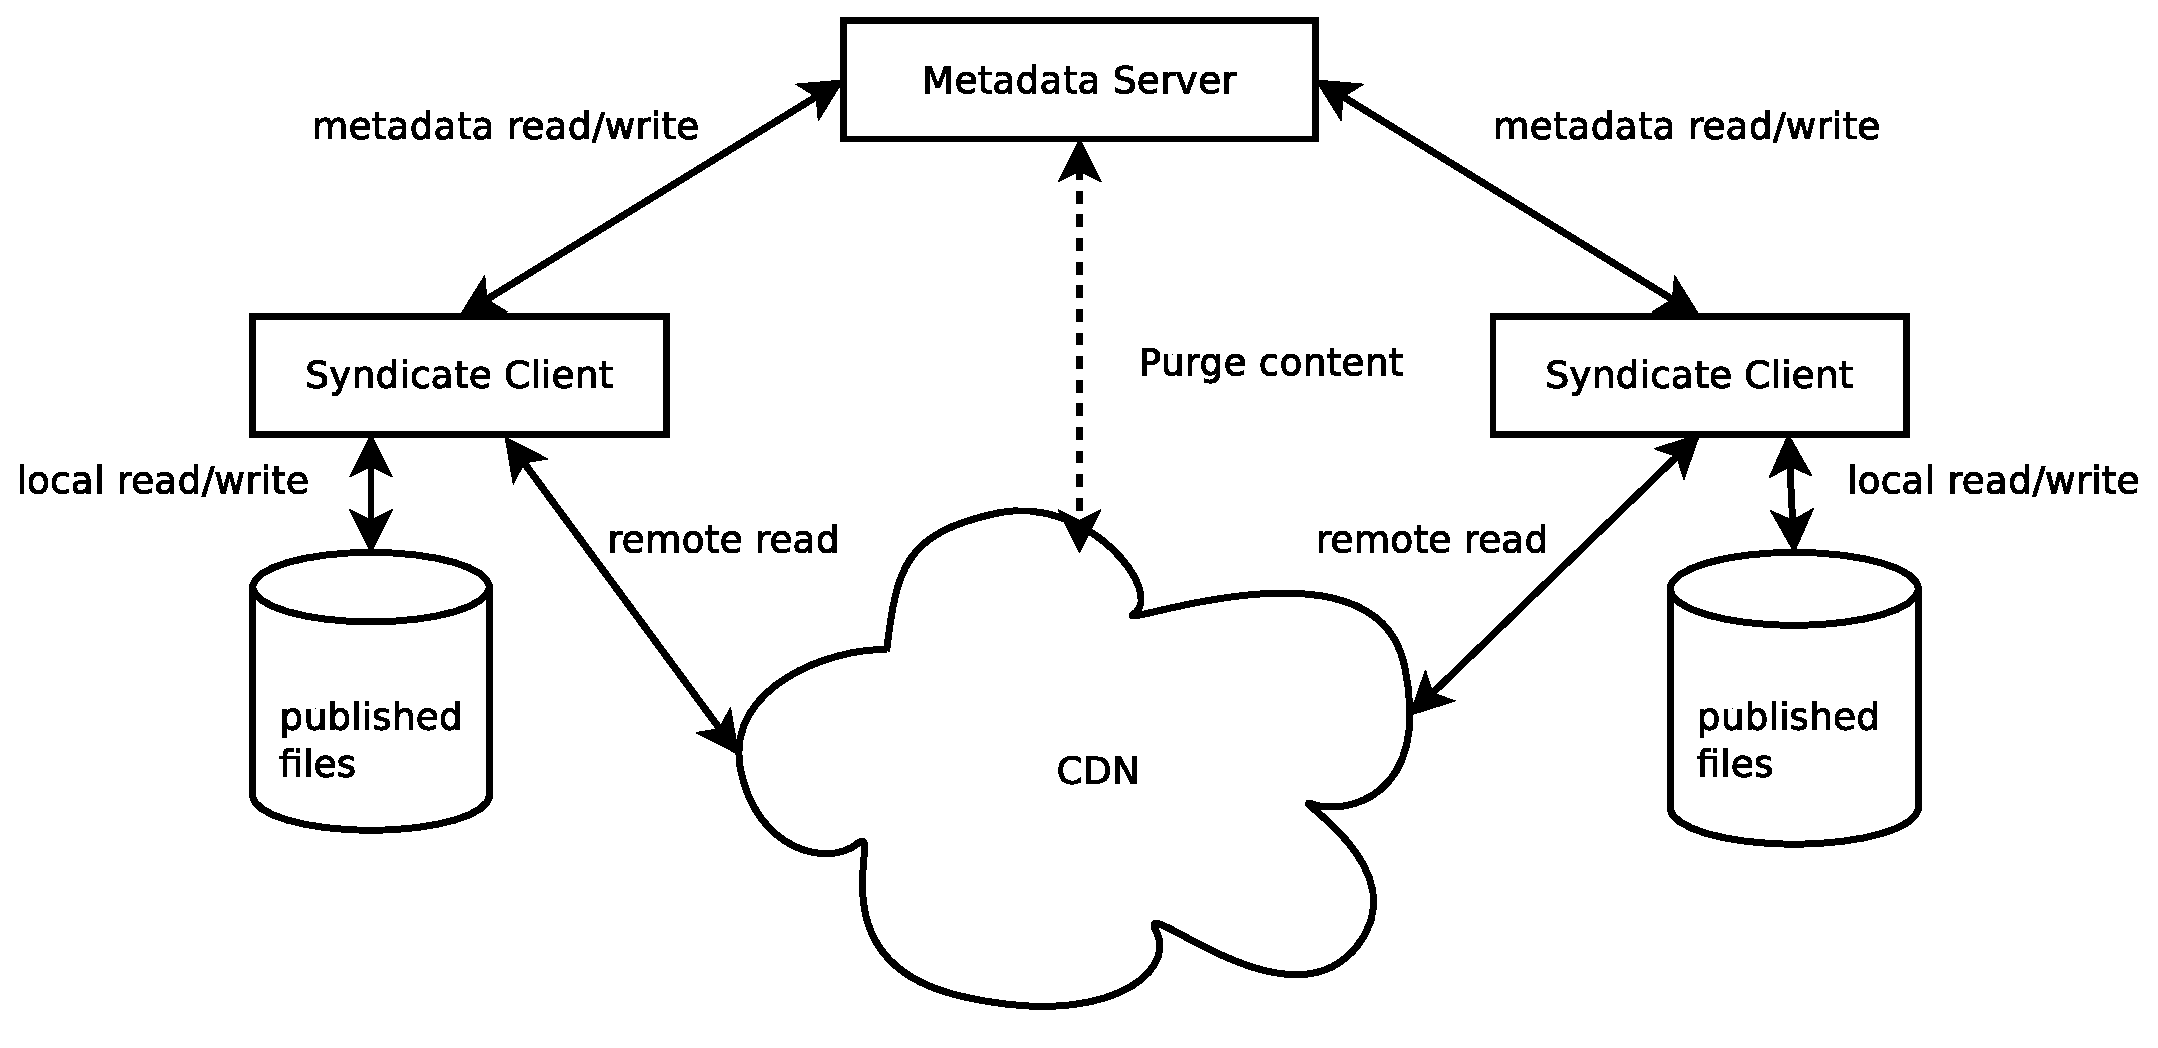
\includegraphics[width=0.5\textwidth]{figures/overview}
\caption{Structural overview of a Syndicate filesystem with two clients.  The ``purge content" operation is an optional CDN feature that Syndicate can use.}
\label{fig:overview}
\end{figure}

% I rewrite the next three paragraphs to describe at a high level the relationship
% between a metadata server and a client.  The metadata server preserves the metadata
% for a filesystem, and the client provides an interface to local processes for manipulating it.
% The client does not enhance the persistence of file data beyond storing locally-created
% data on local storage.  -jcn

Syndicate achieves the semantics of a traditional distributed filesystem despite any immutability
constraints imposed by the CDN by separating the responsibilities of metadata management, 
metadata manipulation, and data distribution.  
A structural overview of a filesystem instance can be seen in Figure~\ref{fig:overview}.
Metadata management is performed by the Syndicate metadata server, which
records metadata changes that occur on files to maintain the authoritive
state of a filesystem's metadata.  Each metadata server uniquely defines
a Syndicate filesystem instance, and relies on clients to upload new metadata
to the authoritive copy on behalf of users.  Logically, we say that a metadata server
implements a Syndicate ``volume" to which clients read and write.

Clients connect to a metadata server to expose its filesystem hierarchy to local processes.
Whenever the client processes a write operation on a file, it generates new
metadata for that file and uploads it to the metadata server to be included 
in the authoritive state.  Then, other clients viewing the same metadata server
will eventually see the effects of the write operation.
The client takes no further action on files written by local processes 
beyond keeping their data on underlying storage.
This data will be served to the CDN for distribution to other clients.

The CDN is responsible for distributing data from hosts with a file's data to
a scalable number of Syndicate clients attempting to read the file.  The CDN does
not need to be designed specifically for Syndicate, but must meet a set of reasonable
architectural requirements to be usable to Syndicate's clients, which we describe
in the next section.  The CDN is invisible to Syndicate users.

When designing Syndicate, we envisioned the most common use-case would be either reading 
and processing remote data as if it were local, or simply to copying remote data to local 
storage (e.g. via "drag-and-drop").  As a result, we optimized Syndicate for read performance, but also
ensured that write performance would be acceptable as long as there were many more readers than writers.

Finally, it is assumed that the clocks on all hosts in a Syndicate filesystem
are loosely synchronized.  In the implementation, we simply run NTPv4 daemons on all hosts to
satisfy this requirement.


\subsection{CDN}
% NOTE: the use of CoBlitz, in my humble opinion, is an implementation detail that should
% be described in the Implementation section.  There would be a subsection that gives an overview
% of why CoBlitz is the best CDN for the job (since it meets these capabilities)

% Syndicate's use of a CDN is agnostic
Our goal in the design of Syndicate's CDN interface is to make Syndicate as CDN-agnostic as possible.  It should treat a CDN as a piece of network infrastructure invisible to users, and make as few assumptions about its behavior as possible.  We describe these minimal assumptions in this section.

% What do we need from our CDN?
First, we assume that all content replicas within the CDN to be addressible by exactly one URL, which we denote $U_{CDN}$.  Syndicate, like a web browser, should not be responsible for tracking individual replicas within the CDN.  We require the CDN to resolve $U_{CDN}$ to an IP address from which to download the bytes of the requested content.

Second, we assume that the CDN identifies a piece of content by its origin URL $U$, and uses an injective function $T$ to map each $U$ to its corresponding $U_{CDN}$.  We require that $T$ be publically known, so Syndicate can resolve a piece of content named by $U$ in the CDN.

Third, we assume that the CDN evicts stale file data on its own. This
includes but is not limited to a least-recently-used cache eviction
policy for infrequently-accessed content.  Syndicate should not be
required to instruct the CDN to remove stale data.

Fourth, we assume the CDN honors a ``do not cache'' hint by not
caching files that Syndicate tags as such.  This is because the
Syndicate client will know immediately when a file has been written
to, and will need to inform the CDN that any data requested from old
URLs to the file should not be stored.

These assumptions are not unreasonable in practice.  CoDeeN~\cite{codeen}, CoralCDN~\cite{coralcdn},
web proxies~\cite{squid}, Amazon Cloudfront~\cite{cloudfront}, and Verivue Hypercache~\cite{vcoblitz} meet
these requirements, for example.

\comment{
Given our assumptions, we construct the Syndicate client to use $T$ to translate any remote file's URL $U$ into $U_{CDN}$ for reading.  We also require the client to generate a new URL to a locally-hosted file whenever it changes, and to be responsible for knowing which URLs to a file refer to stale data.  With these assumptions, we can proceed to design the client to utilize the CDN for file data distribution.
% I also tweaked this last paragraph a bit to make it a bit more clear. -jcn
}

\subsection{Client}

% tasks: present a metadata server's tree, store local files, serve files
The Syndicate client is a filesystem driver.  It generates the
filesystem hierarchy by ``mounting'' a metadata server, which is to say
it authenticates with the metadata server, downloads its filesystem
hierarchy, and periodically refreshes the hierarchy so as to create an
eventually-consistent view of all other files across all other clients
attached to the same metadata server.  The set of metadata attributes
for each file can be found in Table~\ref{tab:metadata-fields}.

% authorization
The client has a Syndicate-wide owner ID used to identify file
ownership.  It occupies the user ID field in a file's entry in the filesystem, but refers
to the client that last wrote to the file (as opposed to the client
that created it).  The owner ID is associated with a user login and
password that the client uses to authenticate with a metadata server,
in order to gain read and write permission and secure metadata
transfer.

The client exposes the metadata server from which it retrieved a file's
metadata in the group ID field.  This ID is unique to a metadata server.
Clients and applications use this field to determine which metadata
server indexes the file data.

File operations are policed using access controls similar to a
conventional UNIX filesystem.  Each file has read, write, and execute
bits for the owner, the users connected to the same metadata server,
and all users in the world.  Both the client and metadata server
restrict access to file data and metadata accordingly, so a rogue user
cannot read or write to the filesystem without proper user credentials
and permissions.

% metadata
\begin{table*}[ht!]
\begin{tabular}{ | l | p{14cm} |}
\hline
\textbf{Name} & \textbf{Description} \\
\hline
\texttt{path} & The path to the file relative to the mountpoint \\
\texttt{url}  & The URL to the file on the origin server (may be a local file URL) \\
\texttt{owner} & The ID of the client that hosts this file \\
\texttt{volume} & The ID of the metadata server that indexes this file \\
\texttt{mode} & UNIX permission bits \\
\texttt{size} & The number of bytes in this file \\
\texttt{mtime} & The time of last modification (seconds) \\
\texttt{atime} & (Clients only) the time of last access (seconds) \\
\texttt{ctime} & (Clients only) the time of file creation (seconds) \\
\texttt{checksum} & Cryptographic hash of the file contents. \\
\hline
\end{tabular}
\caption{Summary of metadata fields kept for each file in the Syndicate filesystem.}
\label{tab:metadata-fields}
\end{table*}

% TODO: do we need a figure of this?  Or is the explanation simple enough to follow?
The client periodically refreshes the metadata by downloading a
directory's metadata from the metadata server if that directory's
entries have changed.  A client can tell when a directory has changed remotely
by downloading the metadata for that directory and comparing its \texttt{checksum} field
against the local version's \texttt{checksum}~\footnote{In practice, the \texttt{checksum} field
of a directory is the cryptographic hash of the name of the directory concatenated with
the names of its entries in alphanumeric order.}.  The locally-unaltered directory entries
are atomically replaced when the directory metadata is refreshed, but uncommitted
local modifications are preserved until the metadata server can be informed of them.
If an entry for a file disappears (e.g. the file was removed or no longer accessible),
the client's underlying storage is unaffected.
Because the client always has file
metadata for each file in the mountpoint, it can trivially service
local metadata read requests.

% remote and local reading
Since a file's metadata includes its web URL, reading a remote file's
data is simply a matter of using $T$ to transform the URL $U$ into
it's CDN-specific URL $U_{CDN}$ and downloading the file from $U_{CDN}
$.  Reads on remote files are synchronous and will block until the
requested data range requested has been fetched (or the download fails
due to an irrecoverable fault).  Whenever a file is downloaded in its
entirety from a read request, the client may optionally calculate a
cryptographic hash of the file data and compare it against the hash
given in the metadata. Then, the read request and all subsequent
read/write operations to that file will fail if the hashes do not
match for as long as the handle to the file is open.  We postpone a more elegant
failure recovery for future work.

As an optimization for remote reads, small and medium-sized files are
downloaded in the background as soon as they are opened and stored
locally until all handles to them are closed. Small files are kept in
RAM, and medium files are kept on local storage.  The size requirements
for ``small'' and ``medium'' are user-defined.


\subsubsection{Underlying Storage}

A Syndicate client access three directories on its local host to expose
filesystem data:  the mountpoint, the \textit{data directory}, and the
\textit{publish directory}.  The data directory is the directory on the
underlying storage that keeps the data for files the client exposes to other clients.  Whenever
a client creates a file in the mountpoint, a corresponding file is created
in the data directory.  Such files are said to be locally-hosted by the Syndicate client.
Read requests from local readers on locally-hosted files are redirected to the
appropriate file in the data directory.

The publish directory stores symbolic links to
files in the data directory, which are then used to generate URLs for locally-created
files.  Symbolic links in the publish directory are appended with version numbers which 
are incremented each time the file it points to is opened, written to, and then closed.

For example, a Syndicate client might be mounted on \texttt{/mnt/syndicate/}, with data directory \texttt{/u/syndicate/}, and publish directory \texttt{/var/www/syndicate/}.  Suppose the client exposes a locally-hosted file at \texttt{/mnt/syndicate/foo/bar/baz}.  Then, its data is stored in \texttt{/u/syndicate/foo/bar/baz}, and it is published at \texttt{/var/www/syndicate/foo/bar/baz.XYZ}, where \texttt{XYZ} is the version number.  If the fully-qualified domain name of the client is \texttt{www.foo.com}, then the file's URL is \texttt{http://www.foo.com/foo/bar/baz.XYZ}.

\subsubsection{Local Writes}

We designed the Syndicate client specifically to avoid the undesired state where
multiple versions of the same file, accessible by the same URL, get cached in 
the CDN.  This is undesired because it may lead to file corruption, depending
on how the CDN reconciles the different versions when it serves them to clients.
This is important because all writes to a locally-hosted in Syndicate are directed to its data in the
data directory.

Every time a locally-hosted file is opened for writing, written to, and closed, the client
\textit{republishes} the file by creating a new symbolic link to it in the 
publish directory.  It gives the symbolic link a greater version number
than all other symbolic links to the modified file.  If the file is deleted locally,
then all symbolic links in the publish directory along with its data in the
data directory will be removed as well.

We assign a new version number to the file whenever it is closed 
(as opposed to written to) for performance reasons.  However, the client
must ensure that between the time when the file is written to and the time
when the file is closed the CDN does not attempt to cache the file.
We do not want the client to ignore requests for this file's data, however, because
a remote reader may still be able to use the data.  So, we have the client
respond to requests for the file with a ``do not cache" tag (in practice, 
the appropriate no-cache HTTP header) so the CDN will not cache different content
for the same URL.

Once the file is closed and republished, the Syndicate client calculates the
new state of its metadata and prepares to send it to the metadata server.
As a performance enhancement, we designed the Syndicate client to buffer
multiple metadata changes and send them in batches.  Once the metadata
server successfully acknowledges the changes, the client removes
the old symbolic links to the modified file.  Then, requests to the stale
URLs they were used to generate will fail, but the metadata changes
(which include the new URLs for the modified files) will eventually propagate
to the other clients, allowing them to read the file once more.  The entire republishing process can be seen in Figure~\ref{fig:write-operation}.

Each metadata change is timestampped by the client so that in the event
that the client cannot quickly upload its changes (e.g. the metadata
server becomes unavailable), the metadata server can still determine to a certain
degree the order in which the client's writes happened with respect to
other clients' writes.  The metadata server uses this timestamp to resolve
write-conflicts.

It is possible for two writers to upload metadata changes for the same file
before seeing the effects of the other's write.  In this scenario, the
client who posted the last write operation (according to the clients' given
timestamps) wins.  To prevent a client from issuing a timestamp far into the
future, the metadata server consequentially ignores changes that
have timestamps that have more than a user-configurable difference from the 
metadata server's local clock.  We detail the process of write-conflict resolution
in the next section.	



\begin{figure}[h!]
\centering
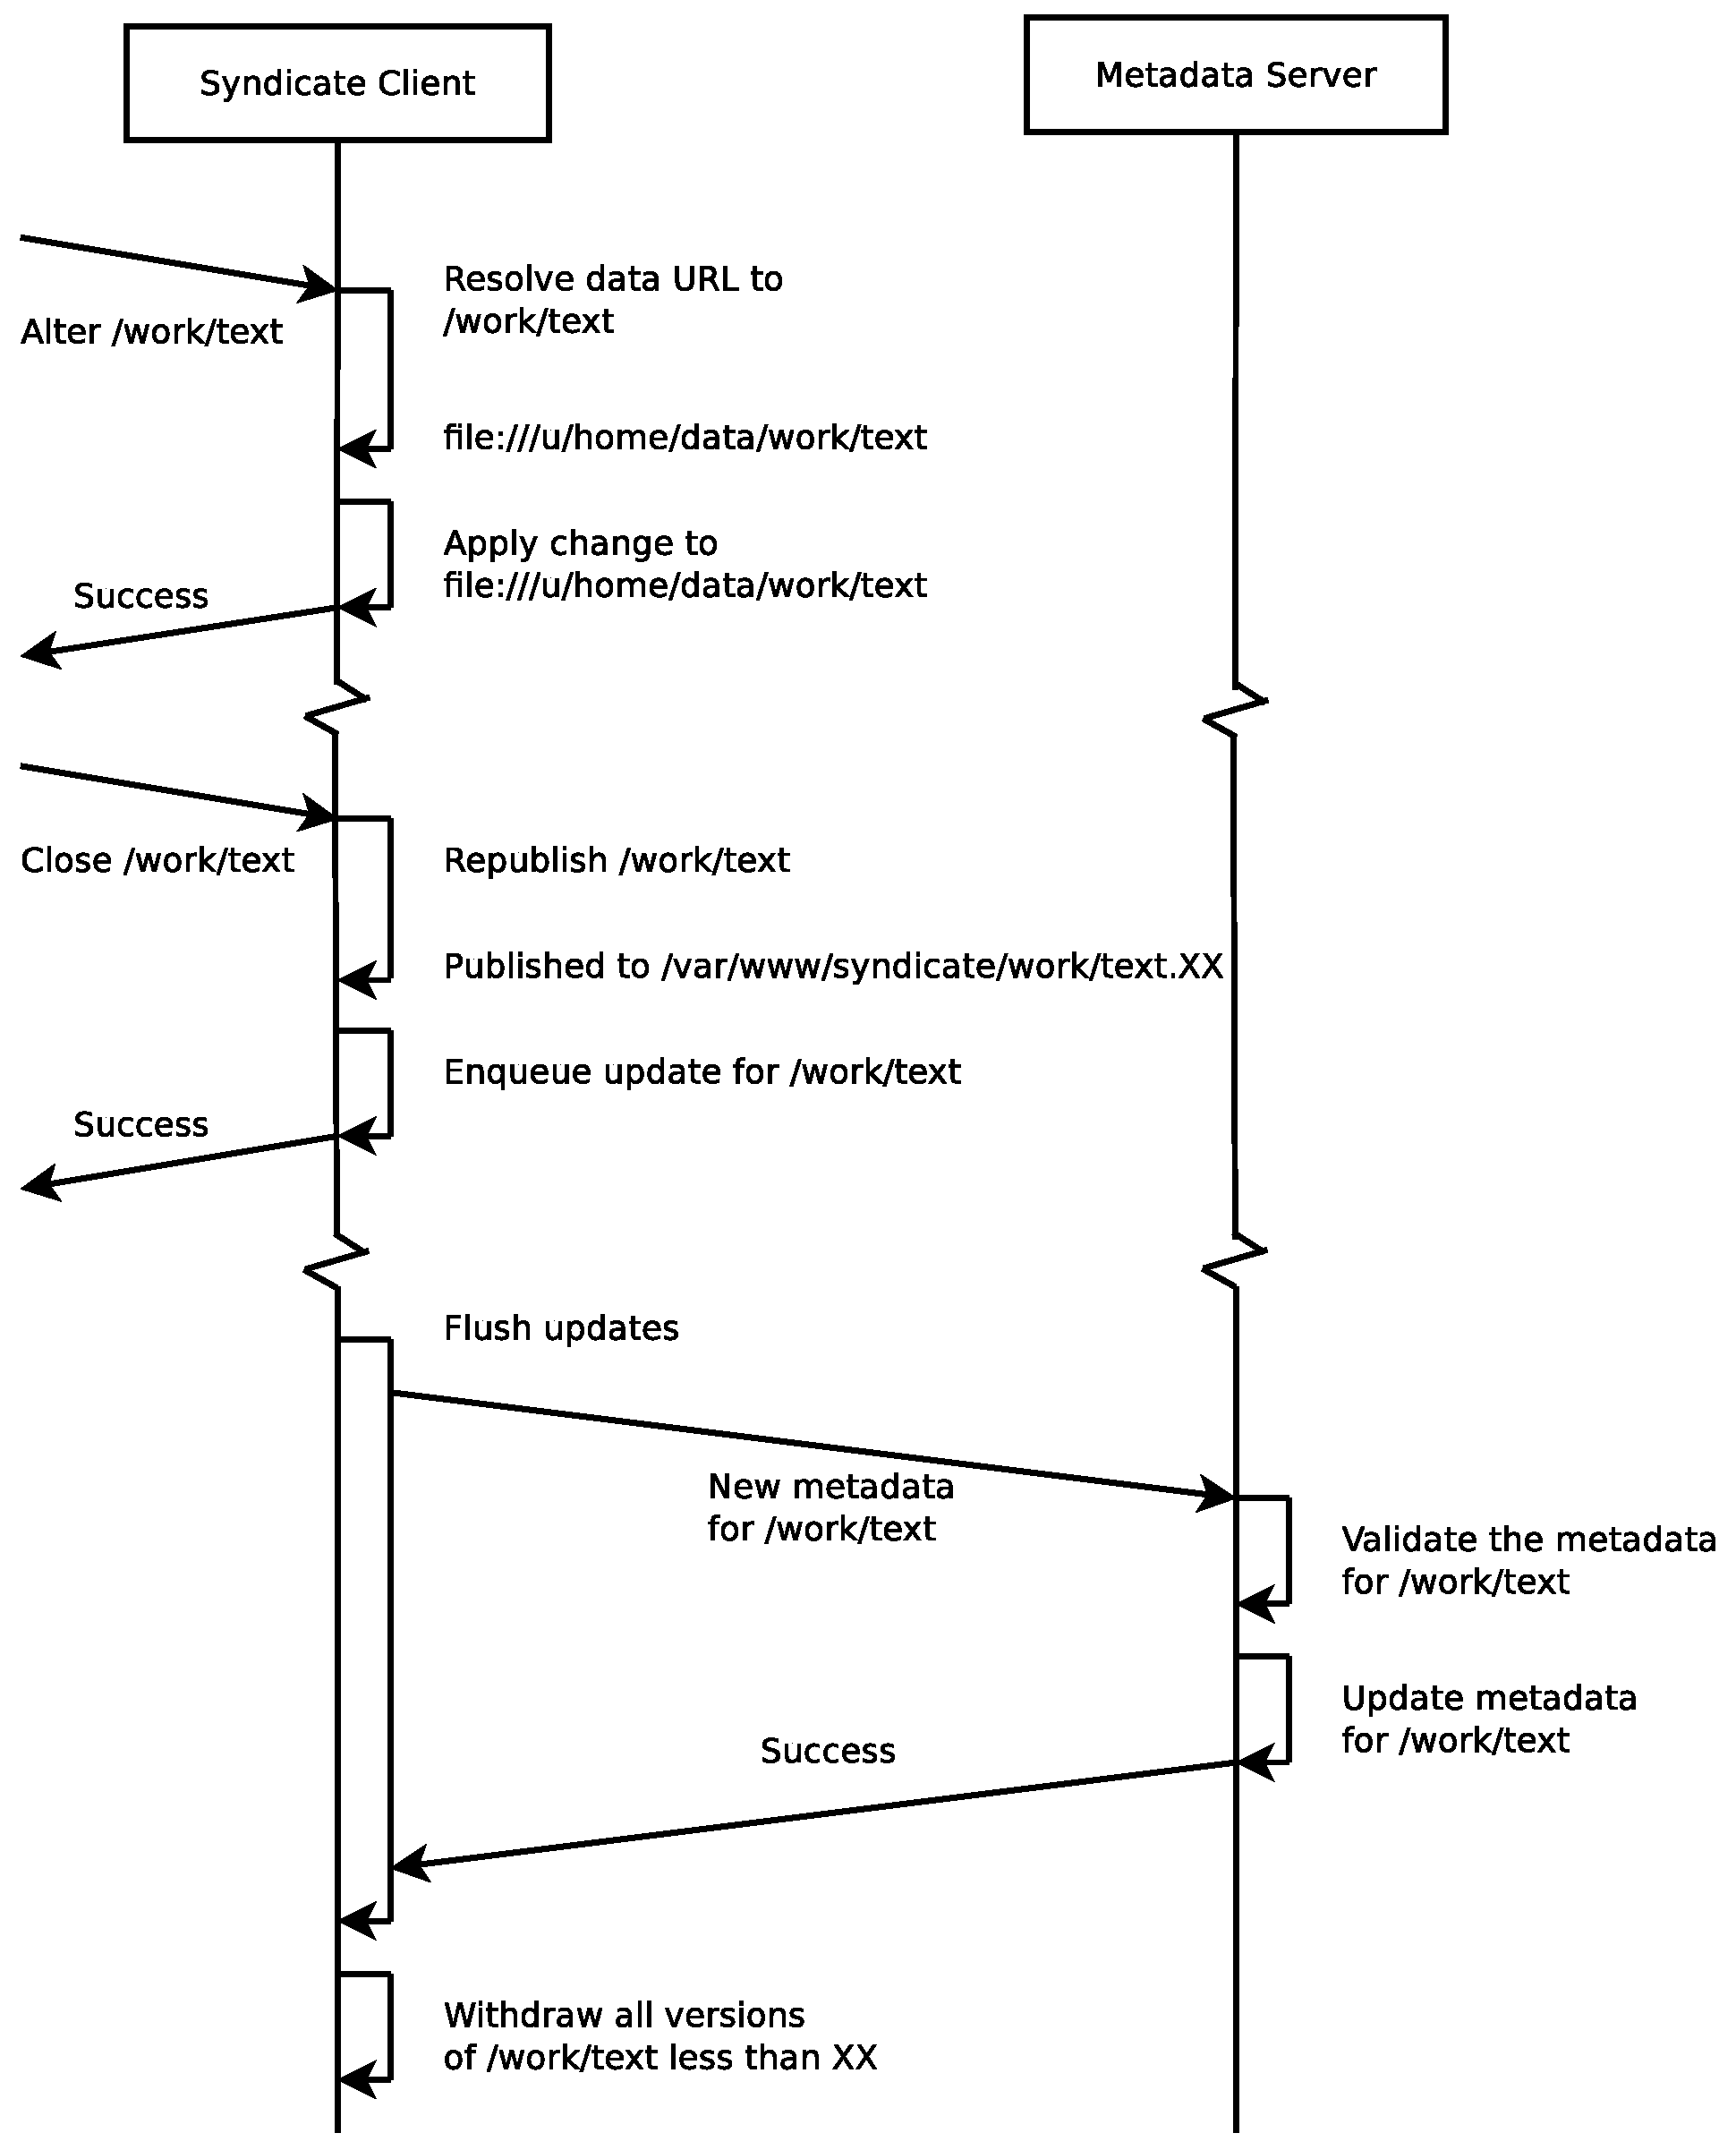
\includegraphics[width=0.5\textwidth]{figures/write-operation}
\caption{The time diagram of writing, closing, and republishing a locally-hosted file \texttt{/work/text}.  The client is mounted on \texttt{/u/home/syndicate/}, and stores local file data in \texttt{/u/home/data/}.  It exposes the data for \texttt{/work/text} in \texttt{/var/www/syndicate/}.  The new version number of \texttt{/work/text} when it is republished is $XX$.}
\label{fig:write-operation}
\end{figure}


\subsubsection{Writing to Remote Content}

% remote file modifications
The client handles a write operation on a remote file by making it a
locally-hosted file first.  It synchronously downloads the file,
optionally verifies its integrity with its metadata's cryptographic
hash, performs the write operation, and republishes it, changing its
owner ID as well.  Future read requests to this file (if no other
changes occur) will now be directed to this client.

% publishing remote files
To publish content from remote sources, the client allows the user to
change the URL of a locally-hosted file by exposing the URL as an
extended file attribute in the filesystem.  This way, a user may
expose data stored on a latency- and bandwidth-constrained remote
medium (such as Amazon S3~\cite{S3}) as a file that can be
distributed to ther clients via the underlying CDN.  This type of
metadata change is propagated to the metadata server as if it were any
other metadata write, but not all metadata fields for this file will
be valid until a client attempts to write to it later (and ends up
hosting the modified copy and generating metadata for it).


\subsection{Metadata Server}

% what does a metadata server do?
The Syndicate metadata server maintains metadata for every file within
its filesystem. It maintains a model of
the entire hierarchy's metadata called the \textit{master copy}.  The
master copy is a filesystem hierarchy with the same directory
structure as will be seen by clients, but each ``file'' is a stub that
contains only its serialized metadata to be served to clients.  The
stub will be regenerated whenever new metadata is uploaded for it by a
client.  The master copy is kept on local storage.
% The reader knows that a metadata server represents a 
% filesystem by now. -jcn

The metadata server is not limited to hosting file metadata for files
hosted on Syndicate clients.  This is because it may be desirable to 
expose content on the Internet as files to clients.  The metadata
server can be programmed to gather metadata for arbitrary Internet
content, and apply a series of user-defined URL rewrite rules to 
transform the content's URL into a path.

% Metadata reading/writing
Each metadata server exports two URLs for its clients: a read URL and
a write URL.  The read URL is used to fetch a directory's metadata
from the master copy, including the metadata for its entries.  Metadata uploaded to the metadata
server via the write URL is validated and committed to the master
copy. A metadata server may optionally require user authentication in
order to gain access to either URL.

% Write conflicts
Each metadata operation is processed in the order in which it arrives,
but conflicting operations are processed in the order of their timestamps.  
If two clients A and B
both perform write operations and commit metadata changes before they observe the other's
write, the metadata change that gets preserved in the master copy will be the metadata
change with the latest timestamp (ties are broken arbitrarily).
Consequentially, a third client C will only see the effects A's or B's writes
(but not both) when it goes to read the file after receiving the new
metadata.  Thus, Syndicate provides at worst close-to-open consistency for
its files, but any client can determine which write succeeded by
inspecting the URL and/or owner ID of a file once the metadata is
refreshed.

% URL blacklisting and validation
URLs in Syndicate may be reused, such as when a file is deleted and
then recreated.  To prevent a file from assuming a URL that refers to
stale data, the metadata server keeps a blacklist of recently stale
URLs which it uses to temporarily block offending metadata writes.  URLs in the
blacklist are removed when the content associated with the URL in the
CDN has been evicted.  This is necessary since the metadata server may
host file metadata for content that changes without the URL changing with it, and should try to prevent
multiple versions of that content from being present on the CDN at one
time.

% Content revalidation
To keep the filesystem consistent over time, the metadata server
periodically revalidates the metadata querying the host of each file in
the master copy order to verify that the file is still available.  If
it is not, then the master copy entry for that file is removed, and the file
entry for it in the clients' mountpoints will disappear when the metadata
is refreshed (unless the file is locally-hosted, in which case the entry
is preserved).  The underlying data on clients is unaffected.
Additionally, the metadata server verifies that each master copy entry
corresponds to the most recent write operation it observed since the
last validation.


\subsection{Fault Tolerance and Failure Modes}

Since clients do not concern themselves with file persistence,
the worst-case effect of a single client failure is that all of the
local files it hosts will no longer be remotely accessible.  They will
temporarily be visible to other clients, but I/O operations that
require the remote client to be contacted will fail with a sensible
error code.  The metadata server will eventually detect that the files
cannot be accessed when it revalidates the metadata, in which case it
removes the file's entry from the master copy.  The local file data
on the inaccessible host will not be affected by this operation.  
%Might be more explicit about reminding the reader we don't guarantee 
%persistence. -llp
% Done.  -jcn

% TODO: make the remount read-only happen
If the metadata server fails, a client's attempts to refresh metadata
will fail.  However, as long as the client runs, it will still provide
a view of the filesystem as it was last known, and for a brief window
of time local write operations will still succeed as far as the
writers are concerned.  Clients will not see the effects of
other clients' writes as long as the metadata server is down, and the
local writes that do succeed will be buffered until they can be sent
off.  The Syndicate client is configured to prevent future writes
whenever it cannot contact the metadata server after a predetermined
timeout in order to warn the user of this failure.

% TODO: make this happen
If the CDN fails to deliver data, all I/O operations on remote files
will fail in every client.  If this happens, a client will fall back to
reading the file directly from the file's remote host instead of going
through the CDN.

\comment{ 
% NOTES

Semantically, you "mount" a metadata server via the Syndicate client.  The metadata server serves the client a filesystem hierarchy of metadata.
\\
The metadata for a file are its relative path, the URL it is available at, its modification time, its owner, its metadata server ID, access mode, size, and (optionally) its cryptographic checksum.
\\
The client creates a filesystem from the metadata and periodically refreshes it.  Agents can query the metadata via the usual syscalls.
\\
Reading a file involves downloading the file from its URL and copying its data into the caller's read buffer when it becomes available.
\\
When a file is created in the filesystem, its data gets stored locally and a version number gets appended to the ``local" path.  The version number is atomically incremented whenever a file handle
to the file that had been opened for writing is closed.
\\
When a file is written to in the filesystem, the file is already hosted locally, or the file is hosted remotely.  If it is local, then the write happens in the
usual way and when the handle is closed the version number gets incremented and the metadata server is informed.
If the file is hosted remotely, the client downloads the file locally and then writes the data to the local copy.
\\
Clients periodically re-download new metadata from the metadata server.
\\
\subsection{Metadata Server}
The metadata server manages the metadata of a filesystem hierarchy.  Whenever a client modifies a file, it uploads the new metadata to the metadata server.
\\
The metadata server performs write-conflict resolution by simply taking the last write to a particular file as the write that succeeded.  
Whenever a client performs a write, the metadata server is informed (since the URL to the file will have changed, since its version number incremented).
\\
The metadata server periodically validates each piece of metadata server by querying each URL for each file and seeing that it is still valid.
\\
\subsection{Content Distribution Network}
TAKEAWAY 1: The reader should have a super-high-level idea of how CoBlitz works, and why now CoBlitz was chosen for our CDN.
\\
Overview of CoBlitz design choices.
\\
CoBlitz nodes cache chunks of requested objects, not the whole object.
\\
CoBlitz replicates chunks between its nodes using highest random weighting.
\\
CoBlitz whitelists clients to contribute to the filesystem.
\\
CoBlitz redirects clients to the appropriate CoBlitz node, based on the requester's location and the health of the nodes.
\\
CoBlitz is already known to be scalable in both the amount of data and number of clients, and has excellent throughput. 
\\
}


